\chapter{System Models}

\section{Scenarios}
The scenarios are based on Node.js based web applications on a server running root and rootJS\\

Web viewer launches and provides a GUI to its end user	\\
Web viewer requests data for visualization by calling rootJS\\
\indent	Node.js invokes ROOT I/O operations\\
\indent \indent		ROOT loads data and provides raw visualization data\\
\indent	Node.js serializes data and streams it to the web viewer\\
Web viewer receives data and renders it in the browser\\
\section{Use Cases}

\pagebreak[4]

\section{Object Models}
Figure 6.1 illustrates what the bindings architecture may look like.
RootApplication::init exposes the available variables, functions and classes via V8 to JavaScript.
Exposed functions call methodProxy, which uses the callee function name to determine the root function that should be called. This will also handle callbacks which are passed wie args parameter.
The classProxy is called instead of methodProxy when the function name is the name of a class and the method therefore is a constructor. This will use ProxyObjectFactory to generate a JavaScript object.
GlobalGetters and Setters is called when a global var should be accessed this again uses the ProxyObjectFactory to generate JavaScript objects.
\\\\
The ProxyObjectFactory creates an instance of a subclass of ProxyObject, the acutal subclass will be decided by using the type parameter.
If the ProxyObject contains a scalar type (like int, long, string, ...) the getV8Handle will simply return the corresponding v8 handle with the value at the defined address.
If the ProxyObject contains an object the getV8Handle method will recursivly call the ProxyObjectFactory for every element it contains and builds a JavaScript object.
To handle reference circles we use a caching mechanism that stores already created v8 handles to reuse them.
\begin{figure}[htb]
	\centering
	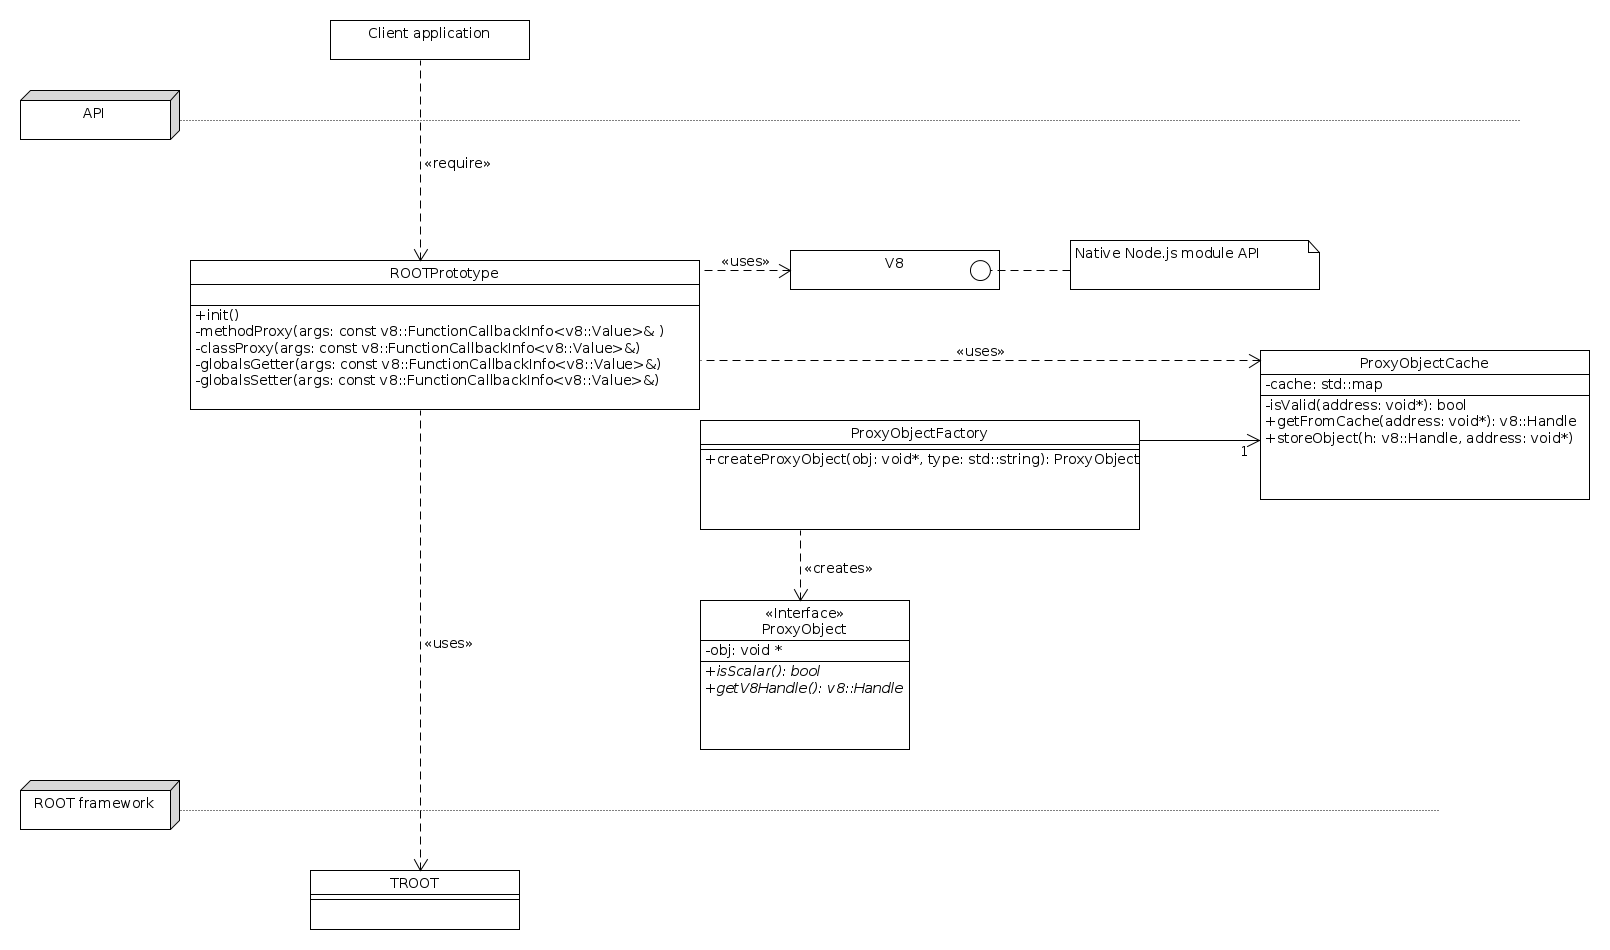
\includegraphics[width=18cm]{./latex/resources/architecture.png}
	\caption{basic architecture draft}
\end{figure}

\pagebreak[4]

\section{Dynamic Models}
The following figure shows how rootJS initializes upon being called the first time by a client application. As bindings do not add any functionality of their own, the client application is not further specified. After the bindings are initialized the client application may use any root functionality through the roootJS API.
\begin{figure}[htb]
	\centering
	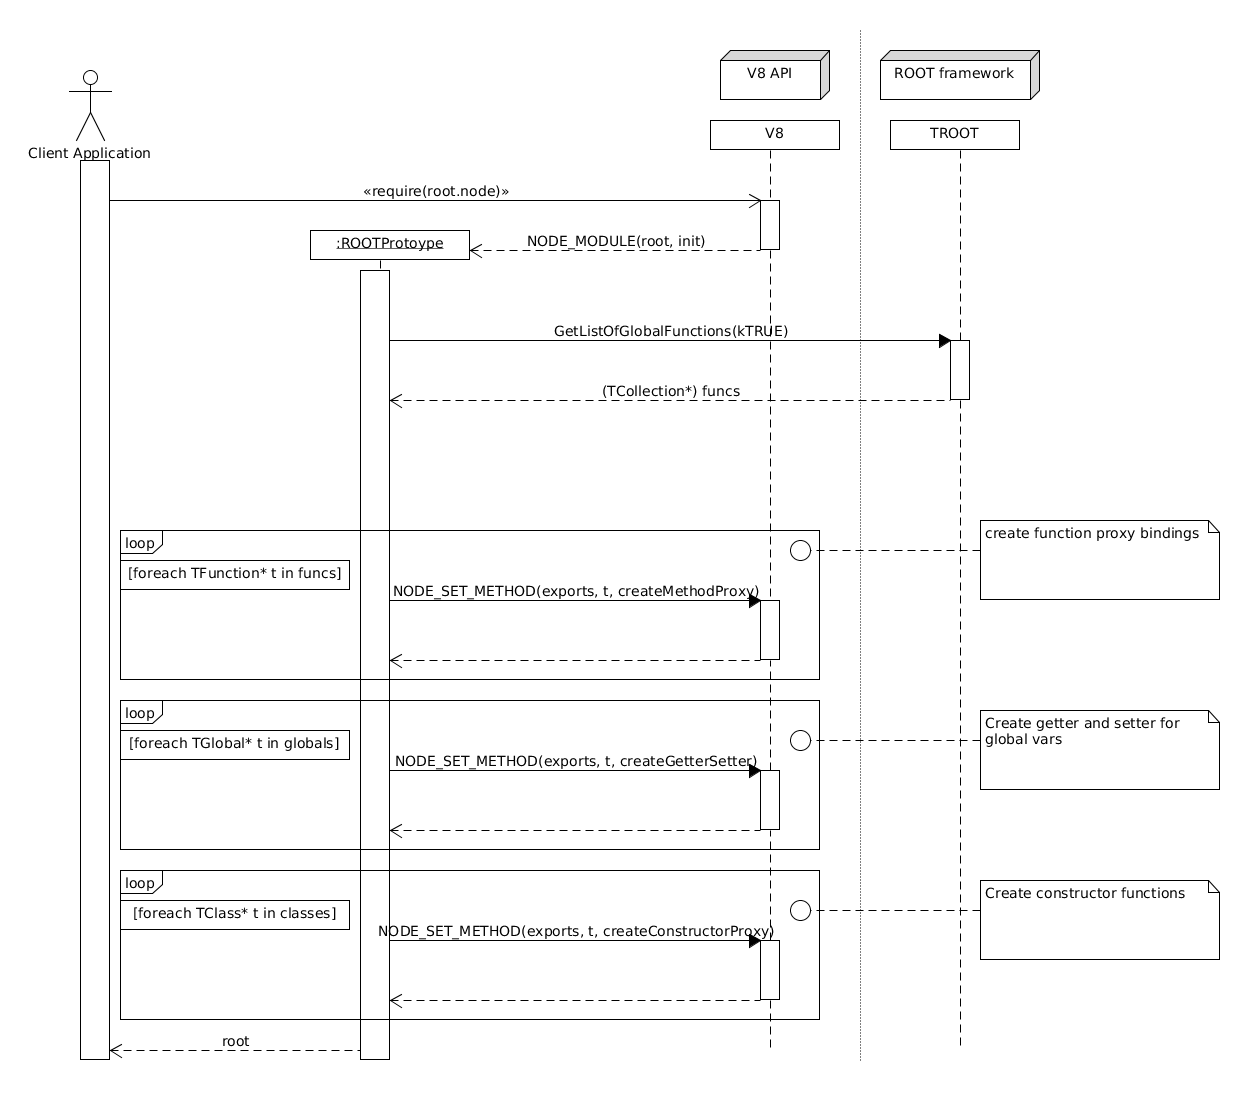
\includegraphics[width=18cm]{./latex/resources/startupSequence.png}
	\caption{startup sequence}
\end{figure}
